\documentclass[10pt,journal,cspaper,compsoc]{IEEEtran}

\usepackage{epsfig}
\usepackage{amssymb,mathrsfs}
\usepackage[cmex10]{amsmath}
\usepackage{theorem}
\usepackage{float}
\usepackage{graphicx}
\usepackage{enumerate}
\usepackage{subfigure}
\usepackage{url}
\usepackage{multirow}
\usepackage{makecell}
\usepackage{color}
\usepackage{balance}
\usepackage{epstopdf}

\usepackage[linesnumbered,vlined,ruled]{algorithm2e}

\interdisplaylinepenalty=2500
\newenvironment{myproof}[1][\proofname]{\proof[#1]\mbox{}}{\endproof}
\newcommand{\blankline}{\vspace*{2ex}}
\newcommand{\remark}[1]{\blankline\noindent\textbf{Remark: }#1}

\newcommand{\argmax}{\mathop{\mathrm{argmax}}}
\newcommand{\pss}{\sigma^2_{\eta_c^i}}
\newcommand{\qss}{\sigma^2_{\eta_c^j}}
\newcommand{\pww}{w^2_i}
\newcommand{\qww}{w^2_j}
\newcommand{\isA}{{\tt isA}}
\newcommand{\cut}[1]{}
\newcommand{\shrink}{\vskip -2ex}
\newcommand{\cwave}{\tilde{c}}

\newtheorem{theorem}{Theorem}
\newtheorem{definition}{Definition}
\newtheorem{property}{Property}
\newtheorem{axiom}{Axiom}
\newtheorem{example}{Example}
\newtheorem{lemma}{Lemma}
\newtheorem{observation}{Observation}
\newtheorem{assumption}{Assumption}
\newtheorem{corollary}{Corollary}

\DeclareMathAlphabet{\mathpzc}{OT1}{pzc}{m}{it}

\begin{document}

\title{Semantic Bootstrapping: A Theoretical Perspective}

\author{Wentao~Wu,
        Hongsong~Li,
        Haixun~Wang,
        and~Kenny~Q.~Zhu% <-this % stops a space
\IEEEcompsocitemizethanks{
\IEEEcompsocthanksitem Wentao Wu is with Microsoft Research, Redmond, WA, USA. E-mail: wentwu@microsoft.com.
\IEEEcompsocthanksitem Hongsong Li is with Microsoft Research Asia, Beijing, China. E-mail: hongsli@microsoft.com.
\IEEEcompsocthanksitem Haixun Wang is with Google Research, Mountain View, CA, USA. E-mail: haixun@google.com.
\IEEEcompsocthanksitem Kenny Q. Zhu, the corresponding author, is with the Department of Computer Science and Engineering, Shanghai Jiao Tong University, Shanghai, China. E-mail: kzhu@cs.sjtu.edu.cn.}
}

\markboth{IEEE Transactions On Knowledge and Data Engineering}
{Wu \MakeLowercase{\textit{et al.}}: Semantic Bootstrapping: A Theoretical Perspective}

\IEEEcompsoctitleabstractindextext{

\begin{abstract}
Knowledge acquisition is an iterative process. Most previous work has focused on bootstrapping techniques based on syntactic patterns, that is, each iteration finds more syntactic patterns for subsequent extraction. However, syntactic bootstrapping is incapable of resolving the inherent ambiguities in the syntactic patterns. The precision of the extracted results is thus often poor. On the other hand, semantic bootstrapping bootstraps directly on knowledge rather than on syntactic patterns, that is, it uses existing knowledge to understand the text and acquire more knowledge. It has been shown that semantic bootstrapping can achieve superb precision while retaining good recall. Nonetheless, the working mechanism of semantic bootstrapping remains elusive. In this paper, we present a detailed analysis of semantic bootstrapping from a theoretical perspective. We show that the efficiency and effectiveness of semantic bootstrapping can be theoretically guaranteed. Our experimental evaluation results substantiate the theoretical analysis.
\end{abstract}

\begin{keywords}
Algorithm, big data, information extraction, semantic bootstrapping
\end{keywords}
}

\maketitle

\section{Introduction}

The problem of extracting \emph{isA} relations in the \emph{open} domain has been studied for years. State-of-the-art systems, such as KnowItAll~\cite{EtzioniCDKPSSWY04}, TextRunner~\cite{BankoCSBE07}, and NELL~\cite{NELL}, use a bootstrapping approach. They start with some seed examples and/or seed patterns of the target relations. They next look for occurrences of these seed examples in the corpus, and derive new patterns. They then use the new patterns to extract more instances of the relations. The iteration continues until no more new patterns are learned. In the rest of this paper, we refer to this idea as \emph{syntactic bootstrapping}. Figure \ref{fig:syntactic} gives a canonical view of this framework.

\begin{figure}[th]
\centering
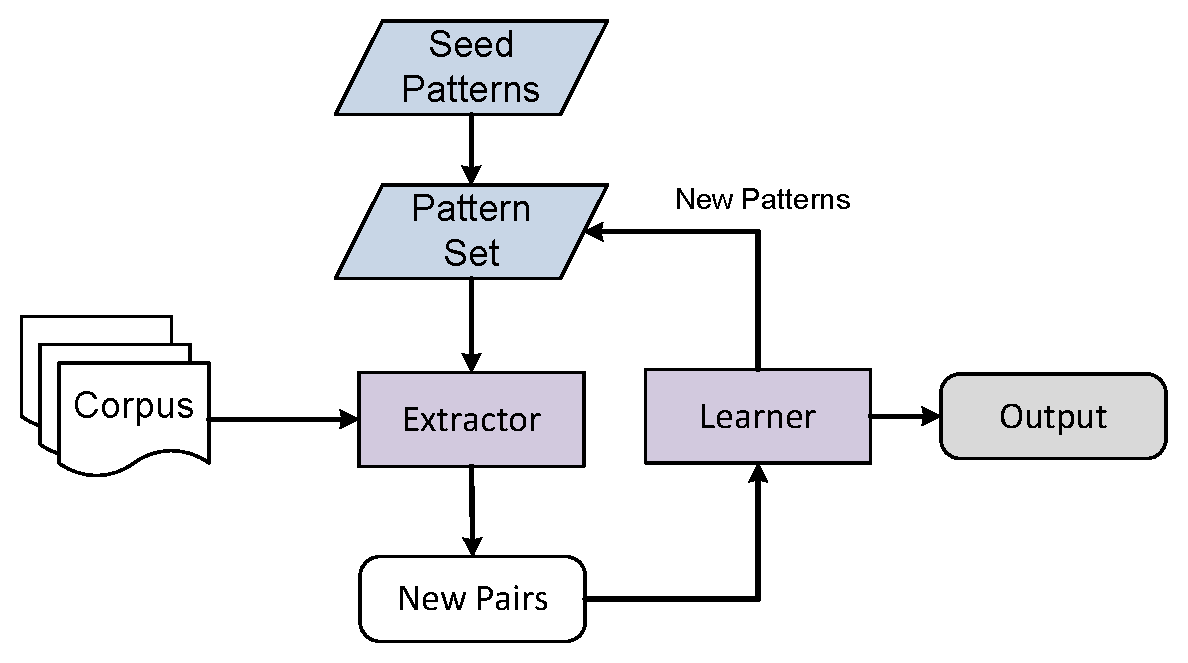
\includegraphics[width=\columnwidth]{syntacticNew2.eps}
\caption{Syntactic bootstrapping}
\label{fig:syntactic}
\shrink
\end{figure}


The philosophy of syntactic bootstrapping is that, in order to find more relations,
we need more syntactic patterns. However, this is often not true. One-to-one mapping between syntactic patterns and underlying \emph{knowledge} (i.e., the pairs we are interested in) does not always exist. Sometimes one pattern can mean multiple things and
multiple patterns can refer to the same thing. This disconnect between
the patterns and knowledge means that acquiring more patterns does not always
give us more knowledge, but rather ambiguity and noise~\cite{WuLWZ12:Probase}.

\begin{table}[!htb]
\small
\centering
\begin{tabular}{|c|c|}
\hline
ID & Pattern \\
\hline
1 & \emph{NP} such as \{\emph{NP},\}$^*$\{(or $|$ and)\} \emph{NP}\\
2 & such \emph{NP} as \{\emph{NP},\}$^*$\{(or $|$ and)\} \emph{NP}\\
3 & \emph{NP}\{,\} including \{\emph{NP},\}$^*$\{(or $|$ and)\} \emph{NP}\\
4 & \emph{NP}\{,\emph{NP}\}$^*$\{,\} and other \emph{NP}\\
5 & \emph{NP}\{,\emph{NP}\}$^*$\{,\} or other \emph{NP}\\
6 & \emph{NP}\{,\} especially \{\emph{NP},\}$^*$\{(or $|$ and)\} \emph{NP}\\
\hline
\end{tabular}
\caption{The Hearst patterns (\emph{NP} stands for \emph{noun phrase})}
\label{tab:hearst}
%\vskip -2ex
\shrink
\end{table}

The problem of ambiguity is ubiquitous in almost all syntactic patterns, even for those hand-crafted by linguistic experts. For instance, Table~\ref{tab:hearst} lists the well-known Hearst patterns~\cite{Hearst92} used by nearly every existing information extraction system for the purpose of extracting \emph{isA} relations. Now consider the following example sentences:

\begin{example} \emph{(Ambiguity in Syntactic Patterns)}
\leavevmode
\label{ex:sentences}
\begin{enumerate}[1)]
\item ... \emph{\underline{animals} other than dogs \textbf{such as}} cats ...
\item ...  \emph{\underline{companies} \textbf{such as}} IBM, Nokia, Proctor and Gamble ...
\item \emph{... representatives in North America, Europe, the Middle East,} Australia, Mexico, Brazil, Japan, China, \emph{{\bf and other} \underline{countries}} ...
\item ... \emph{\underline{classic movies} \textbf{such as}} Gone with the Wind ...
\end{enumerate}
\end{example}
In these cases, patterns are incapable of making the right choices in the presence of ambiguities: 1) {\it dogs} will be incorrectly recognized as the super-concept;\footnote{\emph{isA} relation is between super-concepts and sub-concepts. For example, in the relation ``cat \emph{isA} animal'', ``animal'' is the super-concept and ``cat'' is the sub-concept. In Example~\ref{ex:sentences}, the underlined term is the super-concept, and the italicized terms are its sub-concepts. For a given \emph{isA} relation ($x$, $y$), we also call $x$ the concept and $y$ the instance, although $y$ may itself be a concept as well.} 2) {\it Proctor} and {\it Gamble} are mistakenly extracted as two companies rather than one; 3) {\it North America}, \emph{Europe}, and \emph{the Middle East} will also be deemed as countries; 4) nothing can be extracted since {\it Gone with the Wind} is not a noun phrase that the pattern is looking for.

To address the ambiguity issue, syntactic bootstrapping approaches have to use more strict syntactic rules in their extractions,
which often dramatically sacrifice recall. For instance, when extracting \emph{isA} pairs, KnowItAll only focuses on sub-concepts
that are \emph{proper nouns}~\cite{EtzioniCDKPSSWY04}. Unlike that, in~\cite{WuLWZ12:Probase} the authors outlined a conceptually different iterative framework, which bootstraps on knowledge rather than on syntactic patterns. We refer to this approach as \emph{semantic bootstrapping}.
It differs from syntactic bootstrapping in that it uses a fixed set of input patterns (e.g., the Hearst patterns) and relies on using existing knowledge (e.g., the pairs already extracted with their frequency) to understand more text and acquire more knowledge. 
As Figure \ref{fig:semantic} depicts, in each round of iteration, the extractor extracts new pairs with
the help of the current knowledge, and then uses these new pairs to enrich
the knowledge.
\footnote{
The ``semantic'' here might be a bit misleading.
Our purpose is to distinguish our approach from bootstrapping procedures that aim for harvesting more and more syntactic patterns.
The current form of ``semantic'' in our approach is rudimentary: we simply use statistics as the type of ``semantics'' or ``knowledge.''
Nonetheless, it is not difficult to incorporate more ``semantics'' into our approach.
For instance, we can add annotated \emph{isA} relation pairs to help increase the accuracy of super-concept and sub-concept detection (see Algorithm~\ref{alg:HH2}).
} 
Albeit a simpler framework, this approach demonstrates exceptional strength in disambiguating otherwise unaccessible pairs and thus achieves superb precision while maintaining good recall in the extracted pairs.
\footnote{
Most errors in Example~\ref{ex:sentences} are due to the fact that Hearst-like patterns ignore syntax and syntactic ambiguities. The patterns are flat and not formulated over a parse tree. This raises the question that, if no syntactic ambiguities would exist, would then semantic bootstrapping be obsolete? It is true that using more advanced syntactic techniques such as parser trees might help with some cases, e.g., sentence 1) in Example~\ref{ex:sentences}. However, It cannot address many other cases. For instance, consider sentence 3) in Example~\ref{ex:sentences}.
It does not contain any syntactic ambiguity. Nonetheless, we would end up with incorrect extractions such as (\emph{countries}, \emph{the Middle East}) if we only followed syntactic approaches.
}

\begin{figure}[th]
\centering
\includegraphics[width=\columnwidth]{semanticNew2.eps}
\caption{Semantic bootstrapping}
\label{fig:semantic}
\shrink
\end{figure}

Nonetheless, the underlying working mechanism of semantic bootstrapping remains elusive in~\cite{WuLWZ12:Probase}: were the results reported just by chance? In this paper, we present a theoretical analysis as well as an extended experimental study to provide deeper insights into semantic bootstrapping. We show that the efficiency and effectiveness of semantic bootstrapping can be theoretically guaranteed. Specifically, the required number of iterations is $O(\log |\Gamma|)$, where $\Gamma$ is the set of extracted pairs; and the precision of the extracted pairs is very close to that of the pairs extracted in the bootstrapping stage (i.e., the first two rounds of iterations), which are usually of high quality in practice. Our experimental evaluation results substantiate the theoretical analysis.


\section{Semantic Bootstrapping} \label{sec:extract}

For self-containment purpose, in this section we first formulate the problem of extracting \emph{isA} relations and then briefly describe the semantic bootstrapping framework. We refer the readers to~\cite{WuLWZ12:Probase} for more details of semantic bootstrapping.

\subsection{Problem Formulation}\label{sec:extract:formulation}

\emph{isA} relation can be extracted from sentences that match any of the Hearst patterns, e.g.,\\

``... in \underline{countries} \textbf{such
 as} \emph{China}, \emph{Japan}, ...''\\

Given such a sentence $s$, our goal is then to extract all pairs $(x,y)$ in $s$ such that ``$y$ \emph{isA} $x$''. For instance, from the above sentence, we want to extract ({\em country}, {\em China}) and ({\em country}, {\em Japan}). 
Formally, we can represent $s$ with a triple:
$$s=(X_s,\langle P\rangle,Y_s),$$
where $X_s=\{x_1,...,x_m\}$ is the set of all candidate super-concepts, $\langle P\rangle$ is the pattern keywords (e.g., the ``\textbf{such as}'' in the above example sentence), and $Y_s=\{y_1,...,y_n\}$ is the set of all candidate sub-concepts. %We assume that $\langle P\rangle$ is very unlikely to suffer from the semantic drift problem. Therefore, if $s$ matches $\langle P\rangle$, there is at least one $x\in X_s$ and one $y\in Y_s$ such that ``$y$ \emph{isA} $x$''.
Ideally, we would like both $|X_s|=1$ and $|Y_s|=1$ so that there is no ambiguity. Unfortunately, in practice, this is rarely the case, and our goal is to identify those valid $x$'s and $y$'s among the candidates in $X_s$ and $Y_s$. Here, naturally, we say that a pair $(x,y)$ is valid if the relationship ``$y$ \emph{isA} $x$'' holds. If $(x,y)$ is valid, then both $x$ and $y$ are valid.

\subsection{Properties}\label{sec:extract:properties}

The semantic bootstrapping framework relies on a couple of basic properties of the sentences that match the Hearst patterns to distinguish valid \emph{isA} pairs from invalid ones.

\begin{property}\label{obsv:sup}
For most of the sentences, there is one and only one valid $x\in X_s$.
\end{property}

While in theory the mapping from valid $x\in X_s$ to valid $y\in Y_s$ could be many-to-many, in practice we find it is very unlikely that more than one $x$ in $X_s$ is valid.
Intuitively, if more than one super-concept is valid, then $s$ itself might be too ambiguous to be correctly parsed even by human beings.
In fact, so far we have not even found such a highly ambiguous sentence in our corpus yet.

\begin{property}\label{obsv:sub1}
The closer a $y\in Y_s$ is to $\langle P\rangle$, the more likely that $y$ is valid.
\end{property}

Although it is arguable, we find that when enumerating sub-concepts, people tend to list those that they are familiar with first.

\begin{property}\label{obsv:sub2}
If $y_k\in Y_s$ is valid, then most likely $y_1$, ..., $y_{k-1}$ are all valid.
\end{property}
This means, there is usually a \emph{boundary} in $Y_s$ that delimits valid sub-concepts from invalid ones. For instance, in the sentence 3) of Example~\ref{ex:sentences}, the candidate ``\emph{Australia}'' plays the role of a sentinel.

\remark{
Note that the three properties here are not restricted to \emph{isA} relation extraction. For example, the \emph{authorship} relation can be extracted from sentences like ``\underline{Victor Hugo} \textbf{wrote} \emph{The Hunchback of Notre-Dame} \textbf{and} \emph{Les Mis\'erables}.''
}

In general, as long as we can identify the three components $X_s$, $\langle P\rangle$, and $Y_s$ from a sentence $s$, the above properties are likely to hold and therefore we might be able to apply our semantic bootstrapping framework discussed next. Property~\ref{obsv:sup} usually holds, partially due to the convention when people are writing a sentence. In English grammar, a sentence usually consists of three parts: the \emph{subject}, the \emph{predicate}, and the \emph{object}. For most of the sentences, they only have one subject while they can have multiple objects. Property~\ref{obsv:sub1} and~\ref{obsv:sub2} are usually valid as well, if the sentence contains objects that are chained by using conjunctions such as ``and'' or ``or''. In fact, the pattern ``$y_1$, ..., and/or $y_n$'' occurs very frequently in English documents, and is well known as the \emph{coordination pattern} in the literature~\cite{SnowJN05}.

\subsection{The Algorithm}

Algorithm~\ref{alg:HH2} outlines the method. Here, we use $\Gamma$ to represent the {\em multiset} or {\em bag} of the pairs that we have discovered so far. We also use $\Gamma_i$ to denote the $\Gamma$ after the $i$-th round of iteration in Algorithm~\ref{alg:HH2}, and use $\Delta_i=\Gamma_i - \Gamma_{i-1}$ to denote the multiset of pairs added in round $i$. Initially, $\Gamma_0=\emptyset$. We define a count function $n(x, y)$ which returns how many times the pair $(x,y)$ has been discovered in the corpus.
Initially, $\Gamma$ is empty. We search for candidate pairs in the text, and we use $\Gamma$ to help identify valid ones among them. Specifically, we first call \emph{ExtractCandidates} to extract candidate super-concepts and sub-concepts. The strategy in this stage is rather straightforward: we extract all noun phrases (up to the pattern keywords) as candidates for super-concepts, and we use ``,'', ``and'', and ``or'' as the delimiters for candidate sub-concepts. Next, if $|X_s|>1$, we further call \emph{DetectSuper} to determine the valid super-concept. Once the super-concept is chosen, we can then call \emph{DetectSub} to detect valid sub-concepts. We will discuss some details of these two procedures shortly. 
Finally, we expand $\Gamma$ by merging the newly discovered pairs (line 15).
We keep iterating until we cannot extract any new pairs.

\begin{algorithm}[t]
  \SetAlgoLined
  \KwIn{$P$, the Heast patterns; $S$, sentences that match any of the patterns in $P$}
  \KwOut{$\Gamma$, the extracted \emph{isA} pairs}
  \SetAlgoLined
  $\Gamma \leftarrow \emptyset$\;
  $i\leftarrow 1$\;
  \While {$true$} {
    $\Delta_i \leftarrow \emptyset$\;
    \ForEach {$s \in S$} {
        $X_s, Y_s \leftarrow ExtractCandidates(s)$ \;
        \uIf{$|X_s|>1$}{
          $X_s \leftarrow DetectSuper(X_s, Y_s, \Gamma_{i-1})$\;
        }
        \If{$|X_s|=1$}{
          $Y_s \leftarrow DetectSub(X_s, Y_s, \Gamma_{i-1})$\;
          add valid pairs to $\Delta_i$\;
        }
    }
    break if $\Delta_i=\emptyset$\;
    $\Gamma_i\leftarrow\Gamma_{i-1}\cup\Delta_i$\;
    $i\leftarrow i+1$\;
  }
  \Return{$\Gamma$\;}
  \caption{\emph{isA} relation extraction}
\label{alg:HH2}
\end{algorithm}

\remark{There is a subtle but nontrivial difference between Algorithm~\ref{alg:HH2} and the one described in~\cite{WuLWZ12:Probase}. Note that, in Algorithm~\ref{alg:HH2}, new pairs identified in the current round of iteration are added into $\Gamma$ all together at the end of the round (i.e., \emph{lazy update}), while previously $\Gamma$ was updated immediately when some new valid pair was identified (i.e., \emph{eager update}). Eager update has the advantage of exploiting the new knowledge as soon as possible. As a result, it has the potential to identify more pairs in each round of iteration and therefore speed up the whole extraction procedure. However, it also has a subtle drawback that its results may depend on the order of the input sentences. This is fine if we can always enforce the same ordering, e.g., by sorting the sentences with respect to their unique identifiers or appending new sentences only to the end of the disk file that stores $S$. However, maintenance of $S$ is then costly and might be prohibitive in practice for a frequently updated system like Probase~\cite{WuLWZ12:Probase}. By switching from eager update to lazy update, we can both get rid of the maintenance overhead and the dependency on the input order, although we sacrifice some efficiency by slightly increasing the number of rounds of iteration. Nonetheless, as we will see in Section~\ref{sec:analysis:efficiency}, the efficiency of Algorithm~\ref{alg:HH2} can be theoretically guaranteed. Moreover, we have observed very similar results regarding the precision of the extracted pairs (see Section~\ref{sec:evaluation}).}

\subsection{Super-Concept Detection}

In the case $|X_s|>1$, we need to decide the correct super-concept of $s$. The basic idea is to compute the likelihood $p(x_i|Y_s)$
for each $x_i\in X_s$, and then pick the one with the maximum likelihood. 

Consider $p(x_i|Y_s)$, we have
\begin{equation}
p(x_i|Y_s)\propto p(x_i)p(Y_s|x_i)\propto n(x_i)\prod_{j=1}^{n}p(y_j|x_i).
\end{equation}
Here, we have assumed that the $y_j$'s are independent given $x_i$. Furthermore,
\begin{equation}
p(y_j|x_i)=\frac{p(x_i,y_j)}{p(x_i)}=\frac{n(x_i,y_j)}{n(x_i)},
\end{equation}
where $n(x_i)=\sum_{j=1}^{n}n(x_i,y_j)$. However, if $(x_i,y_j)\not\in\Gamma$, then $n(x_i, y_j)=0$, which implies that a currently unseen pair will make $p(x_i|Y_s)=0$. To overcome this issue, we use the well-known \emph{additive smoothing} technique by refining $p(y_j|x_i)$ as
\begin{equation}
p(y_j|x_i)=\frac{n(x_i,y_j)+\alpha}{n(x_i)+n\alpha},
\end{equation}
where $\alpha>0$ is the smoothing parameter. Therefore,
\begin{eqnarray} \label{eq:bayes-llh}
p(x_i|Y_s)&\propto&\frac{\prod_{j=1}^{n}(n(x_i,y_j)+\alpha)}{(n(x_i)+n\alpha)^{n-1}}.
\end{eqnarray}
Without loss of generality, let $x_1$ and $x_2$ be the candidates with the two \emph{largest} likelihoods such that $p(x_1|Y_s)\geq p(x_2|Y_s)$. We pick $x_1$ as the output of \emph{DetectSuper} if the ratio
\begin{equation}
r(x_1, x_2)=\frac{p(x_1|Y_s)}{p(x_2|Y_s)}
\end{equation}
is greater than some threshold.

\subsection{Sub-Concept Detection}\label{sec:extract:sub-detect}

Assume that we have identified the super-concept $X_s=\{x\}$ from a sentence. The next task is to find its sub-concepts from $Y_s$. Based on Property~\ref{obsv:sub1} and~\ref{obsv:sub2}, the strategy is to first find the \emph{largest} scope wherein candidate sub-concepts are all valid, and then address the ambiguity issues inside the scope by using a similar likelihood-based approach to the one used in super-concept detection. Specifically, we find the largest $k$ such that the likelihood
$p(y_k|x)$ is above a threshold. On the other hand, if we cannot find any $y_k$ satisfying the condition, then
we assume $k=1$, provided that $y_1$ is not ambiguous (i.e., it
does not contain ``and'' or ``or'').

\begin{example}[Sub-Concept Detection]
\label{ex:detect-sub}
For specificity let us again consider sentence 3) in Example~\ref{ex:sentences}. In terms of the problem formulation as was presented in Section ~\ref{sec:extract:formulation}, we have $X_s=\{$countries$\}$ and $Y_s=\{$North America, Europe, the Middle East, Australia, Mexico, Brazil, Japan, China$\}$. We expect that (countries, Australia) has significantly higher likelihood than (countries, the Middle East). As a result, ``Australia'' serves as the boundary in $Y_s$, and \emph{DetectSub} would extract ``Australia,'' ``Mexico,'' ``Brazil,'' ``Japan,'' and ``China'' from the sentence.
\end{example}

\section{Efficiency}\label{sec:analysis:efficiency}

In this section, we analyze the efficiency of Algorithm~\ref{alg:HH2}. Since the total number of pairs we can extract from the corpus is finite, and in each round we only add new valid pairs extracted from the sentences into $\Gamma$, Algorithm~\ref{alg:HH2} is guaranteed to terminate. The efficiency depends on the number of iterations it executes. In the following presentation, we say a sentence $s$ in round $i$ is \emph{ambiguous} if $|X_s|>1$ \emph{after} applying \emph{DetectSuper}, and \emph{unambiguous} otherwise.

Before we proceed, we first redefine the notation $S$ to be the set of sentences we finally extract \emph{at least one} pair, not the set of all sentences in our corpus. In practice, it is likely that we cannot extract any pair from some sentences. For example, if we finally cannot determine the correct super-concept of a sentence, then we fail to extract anything from it. These sentences do not contribute anything to our results, so we exclude them from our analysis below.

\begin{table}[h]
\small
\centering
\begin{tabular}{|c|l|}
\hline
Notation & Description \\
\hline
$\Gamma_i$ & All pairs extracted \emph{after} iteration $i$\\
$\Delta_i$ & The pairs extracted \emph{in} iteration $i$\\
$\Omega_i$ & The remaining pairs in $\Gamma$ after iteration $i$\\
$\bar{L}_i$ & \makecell[l]{The average number of pairs that can be\\ extracted from a sentence after iteration $i$}\\
$\sigma_i^x$ & \makecell[l]{The probability that some $y\in\Delta_i^x$\\ becomes a new boundary sub-concept}\\
$P_i$ & The precision of pairs in iteration $i$\\
\hline
\end{tabular}
\caption{Notation used in the analysis of Algorithm~\ref{alg:HH2}}
\label{tab:notation}
\shrink
\end{table}

Our analysis of the number of iterations is based on the analysis of expected number of pairs that can be extracted in each iteration.
We find that the latter shrinks exponentially as the iteration proceeds, which therefore implies a logarithmic convergence speed of the extraction procedure.
For convenience of reference, we summarize the key notation used in our analysis in Table~\ref{tab:notation}.
We start our analysis by presenting a basic property of \emph{DetectSub}.

\subsection{A Basic Property of \emph{DetectSub}}

Consider an arbitrary sentence $s$ in round $i+1$. Note that if $s$ is ambiguous in round $i+1$, then we cannot extract any pair from it. Hence we only need to focus on the case when $s$ is unambiguous. Let $x$ be the super-concept of $s$, and $Y_s=\{y_1, ..., y_n\}$. Assume that $y_1,...,y_j$ have been detected by \emph{DetectSub} before round $i+1$. Then we can extract some pair(s) from $s$ in round $i+1$ only if there is some $k$ ($j<k\leq n$) such that $y_k$ can be identified by \emph{DetectSub}.
Note that we seek the maximum $k$ in \emph{DetectSub}, and all $y_{j+1}$ to $y_k$ will be extracted once $y_k$ is identified. Therefore, we refer to $y_k$ as the current \emph{boundary} sub-concept of $s$. We have the following property for $y_k$.

\begin{lemma}\label{lemma:yk}
$(x,y_k)\in\Delta_i$, where $\Delta_i=\Gamma_i-\Gamma_{i-1}$.
\end{lemma}

\begin{proof}
Let $p_i(y_k|x)$ be the value of the likelihood $p(y_k|x)$ that \emph{DetectSub} is concerned with in round $i$. If $(x,y_k)\not\in\Delta_i$, then $n(x,y_k)$ does not change between round $i$ and $i+1$. Hence, $p_{i+1}(y_k|x)\leq p_i(y_k|x)$. Since we failed to extract $(x,y_k)$ from $s$ in round $i$ only if $p_i(y_k|x)<\epsilon$, we must have $p_{i+1}(y_k|x)<\epsilon$ as well. Here $\epsilon$ is the threshold. Therefore, $y_k$ cannot be identified by \emph{DetectSub}, a contradiction.
\end{proof}

Lemma~\ref{lemma:yk} basically states that, if $y_k$ could be a boundary sub-concept, then its frequency (i.e., $n(x, y_k)$) must have been changed in round $i$ (i.e., $(x,y_k)\in\Delta_i$). Therefore, when searching for a potential boundary sub-concept in round $i+1$, we can just focus on such $y_k$'s.
Based on this observation, we next analyze the expected number of pairs that can be extracted in each round.

\subsection{The Expected Number of Extracted Pairs}

We further break down our analysis here into two smaller steps. For a given sentence, we are interested in the following two questions:
\begin{itemize}
    \item What is the likelihood that we can extract at least one pair from it? We call this likelihood the \emph{chance of success}.
    \item What is the expected number of extracted pairs given that we can extract at least one pair from it? We call this expectation the \emph{expected successes}.
\end{itemize}
We next analyze these two problems one by one.

\subsubsection{The Chance of Success}

Define $\Delta_i^x$ to be the set of pairs in $\Delta_i$ with $x$ the super-concept. Based on Lemma~\ref{lemma:yk}, the possible boundary $y_k$ can only come from $\Delta_i^x$. We assume that each distinct $y$ in $\Delta_i^x$ is equally likely to be this $y_k$, with some probability $\theta$ ($0<\theta<1$). Of course, for different $s$, $\theta$ may be different. So here $\theta$ should be viewed as the average over all sentences.
$\theta$ may also depend on the round number $i$. We give some further analysis here. Note that $\theta$ is the probability of the event $E_y$: ``$y\in\Delta_i^x$ is a new boundary $y_k$ in round $i+1$ for $s$''. $E_y$ occurs if and only if the following two events occur:
\begin{itemize}
\item $E_y^1$: $j<k\leq n$, i.e., the new boundary should bring in at least one new sub-concept.
\item $E_y^2$: $p(y_k|x)\geq\epsilon$, i.e., the new boundary should pass the likelihood threshold $\epsilon$.
\end{itemize}
Assuming the independence of $E_y^1$ and $E_y^2$, we have $\theta=p(E_y)=p(E_y^1)p(E_y^2)$. On one hand, as the iteration proceeds, $p(E_y^1)$ is expected to decrease, since it is more and more difficult to identify new sub-concepts from a sentence given that the total number of valid sub-concepts in a sentence is fixed. On the other hand, $p(E_y^2)$ is expected to increase, since $\Gamma$ keeps on growing and the count of a valid pair is increasing as well. We thus treat $\theta$ as a constant.

For the ease of exposition, we formalize this assumption in the following:
\begin{assumption}\label{assumption:uniform}
Each distinct $y\in\Delta_i^x$ is independently and equally likely to be the boundary sub-concept $y_k$, with probability $\theta$.
\end{assumption}
We note here that this assumption may not be valid in reality. It is certainly possible that some sub-concepts are more likely than the others to be the boundary. However, Assumption~\ref{assumption:uniform} is reasonable if we do not have any \emph{prior} knowledge on which sub-concepts are more likely, according to the principle of maximum entropy. On the other hand, if we do have such prior knowledge, we may replace this ``uniform distribution'' assumption by the real distribution, which is a possible extension to the current framework.

Let $D(\Delta_i^x)$ be the set of distinct $y$'s in $\Delta_i^x$.
Consider the probability $\sigma_i^x$ that some $y\in D(\Delta_i^x)$ becomes a new boundary of $s$.
By Assumption~\ref{assumption:uniform}, the probability that none of the $y$'s in $D(\Delta_i^x)$ can be a new boundary is then $(1-\theta)^{|D(\Delta_i^x)|}.$ Define $q=1-\theta$. We have
\begin{equation}\label{eq:sigmaix}
\sigma_i^x=1-(1-\theta)^{|D(\Delta_i^x)|}=1-q^{|D(\Delta_i^x)|}.
\end{equation}

\subsubsection{The Expected Successes}

Suppose that we can identify some new boundary of $s$. Let $\bar{L}_i$ be the average number of pairs that can be extracted from a sentence after round $i$. Similar to Assumption~\ref{assumption:uniform}, we have the following assumption:
\begin{assumption}\label{assumption:uniform2}
Each of $y_{j+1}$, ..., $y_n$ is equally likely to be the $y_k$ with the largest $k$ determined by \emph{DetectSub}.
\end{assumption}
The expected number of pairs extracted from $s$ in round $i+1$ is then
\begin{equation}\label{eq:avglen}
E[L_{i+1}^s]=\frac{1}{\bar{L}_i}(1+\cdots+\bar{L}_i)=\frac{1}{2}(1+\bar{L}_i).
\end{equation}
Equation~\ref{eq:avglen} may be worth some further explanation. Consider the following example:
\begin{example}
Let $s$ be ``$x$ such as $y_1$, $y_2$, and $y_3$.''
Then $\bar{L}_0 = 3$, assuming that $s$ is the only sentence in $S$. Note that $\bar{L}_0$ is unknown to \emph{DetectSub}.
So by Assumption~\ref{assumption:uniform2}, \emph{DetectSub} may extract $1$, $2$, or $3$ sub-concepts, depending on which of $y_1$, $y_2$, and $y_3$ is determined to be the boundary sub-concept. The expected number of extracted sub-concepts is therefore $E[L_1]=\frac{1}{3}(1 + 2 + 3) = 2$.
\end{example}

\subsubsection{Putting It Together}

We are now ready to compute the number of expected pairs extracted in each round.
Let $\Omega_i=\Gamma-\Gamma_i$, which is the \emph{remaining} pairs in $\Gamma$ that can be extracted \emph{after} round $i$. As before, let $\Omega_i^x$ be the subset of $\Omega_i$ containing pairs with $x$ the super-concept. Our next result shows that the number of remaining pairs decreases exponentially as the iteration proceeds:

\begin{lemma}\label{lemma:Omega}
$|\Omega_{i+1}^x|<\gamma_i^x|\Omega_i^x|$, where $\gamma_i^x=\frac{1}{2}(1+q^{|D(\Delta_i^x)|})$.
\end{lemma}

\begin{proof}
By the definition of $\Omega_i$, we have 
\begin{equation}
|\Omega_i^x|=\bar{L}_i|S^x|,
\end{equation}
where $S^x$ is the subset of $S$ containing sentences with $x$ the super-concept. 
By Equation~\ref{eq:avglen}, the number of pairs we expect to extract in round $i+1$ is 
\begin{equation}
E[L_{i+1}^x]=\frac{1}{2}(1+\bar{L}_i)|S^x|. 
\end{equation}
Thus the expected number of remaining pairs after round $i+1$ is then
\begin{eqnarray}\label{eq:omegax}
|\Omega_{i+1}^x|&=&|\Omega_i^x|-E[L_{i+1}^x]\cdot\sigma_i^x\\\nonumber
&=&\bar{L}_i|S^x|-\frac{1}{2}(1+\bar{L}_i)|S^x|\cdot\sigma_i^x\\\nonumber
&=&\big[(1-\frac{1}{2}\sigma_i^x)\bar{L}_i-\frac{1}{2}\sigma_i^x\big]|S^x|\\\nonumber
&<&(1-\frac{1}{2}\sigma_i^x)\bar{L}_i|S^x|.
\end{eqnarray}
Hence we now have
\begin{equation}
|\Omega_{i+1}^x|<(1-\frac{1}{2}\sigma_i^x)|\Omega_i^x|=\frac{1}{2}(1+q^{|D(\Delta_i^x)|})|\Omega_i^x|,
\end{equation}
which completes the proof of the lemma.
\end{proof}

\remark{We have two remarks here for Lemma~\ref{lemma:Omega}.
First, for a particular $x$, the specific value of $\gamma_i^x$ depends on the number of pairs in $\Delta_i^x$.
Since $q<1$, $q^{|D(\Delta_i^x)|}$ can be ignored even for a very small $\Delta_i^x$ with only dozens of distinct pairs.
Therefore, we can actually expect $|\Omega_{i+1}^x|<\frac{1}{2}|\Omega_i^x|$ for most of the rounds except for the last few ones.
Thus, usually we can grab more than half of the remaining pairs in each round.
Second, different $x$ has different $|D(\Delta_i^x)|$, and hence has different $\gamma_i^x$.
As discussed above, $\gamma_i^x\approx\frac{1}{2}$ unless $|D(\Delta_{i}^x)|$ is very small.
In practice, it is well known that most pairs in $\Omega_i$ are from a small number of $x$'s. These $x$'s usually have large $D(\Delta_{i}^x)$.
Since $|\Omega_{i+1}^x|<\frac{1}{2}|\Omega_i^x|$ for these $x$'s, we can also expect $|\Omega_{i+1}|<\frac{1}{2}|\Omega_i|$ (except for the last several rounds).
}

\subsection{The Convergence Rate of Algorithm~\ref{alg:HH2}}

It is now easy to prove the following theorem, which basically states that Algorithm~\ref{alg:HH2} will converge in logarithmic rate with respect to $|\Gamma|$.
This is a natural corollary from Lemma~\ref{lemma:Omega}.

\begin{theorem}\label{theorem:convergence}
Algorithm~\ref{alg:HH2} is expected to end after $\lceil\log_{\frac{1}{\gamma}}|\Gamma|\rceil+1$ rounds of iteration, where $\gamma=\frac{1}{2}(1+q)$.
\end{theorem}

\begin{proof}
Based on Lemma~\ref{lemma:Omega},
\begin{equation}
|\Omega_{i+1}^x|<\frac{1}{2}(1+q^{|D(\Delta_i^x)|})|\Omega_i^x|,
\end{equation}
for a specific $x$. Since $q<1$ and $|D(\Delta_i^x)|\geq 1$, we have
\begin{equation}
|\Omega_{i+1}^x|<\frac{1}{2}(1+q)|\Omega_i^x|=\gamma|\Omega_i^x|.
\end{equation}
Note that this is true regardless of the $x$. Therefore,
\begin{equation}
|\Omega_{i+1}|<\frac{1}{2}(1+q)|\Omega_i|,
\end{equation}
since $|\Omega_i|=\sum_{x}|\Omega_i^x|$. After $N$ rounds of iteration, the number of remaining pairs that can be extracted is 
\begin{equation}
|\Omega_N|< \gamma^{N-1}|\Omega_1| < \gamma^{N-1}|\Gamma|.
\end{equation}
Since $q<1$, we must have $\gamma=\frac{1}{2}(1+q)<1$. Letting $\gamma^{N-1}|\Gamma| < 1$ gives us that $N > \log_{\frac{1}{\gamma}}|\Gamma|+1$. This means, after $N'=\lceil\log_{\frac{1}{\gamma}}|\Gamma|\rceil+1$ rounds, it is expected that $|\Omega_{N'}|<1$. 
Algorithm 1 cannot extract more pairs and hence terminates.
\end{proof}


\section{Precision}\label{sec:analysis:precision}

In this section, we analyze the precision of the pairs extracted by Algorithm~\ref{alg:HH2}. Since precision can only be manually evaluated, our goal here is not to give an explicit number. Rather, we develop a lower bound of the expected overall precision given that the precision of the first several rounds is known. Specifically, our analysis shows that the overall precision only depends on the precision of the pairs extracted in the first two rounds. Since in practice the precision of these pairs is usually very high, we can therefore expect high precision of all the pairs extracted.

In the following, we start by giving a representation of the total number of extracted pairs (i.e., $|\Gamma|$). Our analysis shows that $|\Gamma|$ can be approximately expressed in terms of the number of pairs extracted in the first two iterations. We then conduct a similar study on the total number of \emph{correct} pairs extracted, which again connects it with the number of \emph{correct} pairs extracted in the first two iterations. As a final step, we develop an expression for the overall precision based on the previous two results, and further derive a natural lower bound according to the established expression. Again, we refer the readers to Table~\ref{tab:notation} for the key notation used in this section.

\subsection{The Total Number of Extracted Pairs}

We first analyze the relationships between the $|\Delta_i^x|$'s, i.e., the number of pairs extracted in each round with $x$ the super-concept. We have the following lemma:
\begin{lemma}\label{lemma:Delta}
Let $N$ be the number of rounds Algorithm~\ref{alg:HH2} iterates before its termination. Then
\begin{equation}
\sum_{j=1}^{N}|\Delta_j^x|=|\Delta_1^x| + \frac{2}{1-q^{|D(\Delta_1^x)|}}|\Delta_2^x|-|S^x|.
\end{equation}
\end{lemma}

\begin{proof}
In the proof of Lemma~\ref{lemma:Omega}, we have shown
\begin{equation}
|\Omega_{i+1}^x|=\big[(1-\frac{1}{2}\sigma_i^x)\bar{L}_i-\frac{1}{2}\sigma_i^x\big]|S^x|.
\end{equation}
Since $|\Omega_i^x|=\bar{L}_i|S^x|$, the above can be rewritten as
\begin{equation}
|\Omega_{i+1}^x|=(1-\frac{1}{2}\sigma_i^x)|\Omega_i^x|-\frac{1}{2}\sigma_i^x|S^x|.
\end{equation}
Since $|\Delta_{i+1}^x|=|\Omega_i^x|-|\Omega_{i+1}^x|$, it follows that
\begin{equation}
|\Delta_{i+1}^x|=\frac{1}{2}\sigma_i^x|\Omega_i^x|+\frac{1}{2}\sigma_i^x|S^x|.
\end{equation}
Note that $|\Omega_i^x|=\sum_{j=i+1}^{N}|\Delta_j^x|$, which gives
\begin{equation}
|\Delta_{i+1}^x|=\frac{1}{2}\sigma_i^x\sum_{j=i+1}^{N}|\Delta_j^x|+\frac{1}{2}\sigma_i^x|S^x|,
\end{equation}
or equivalently,
\begin{equation}
(1-\frac{1}{2}\sigma_i^x)|\Delta_{i+1}^x|=\frac{1}{2}\sigma_i^x\sum_{j=i+2}^{N}|\Delta_j^x|+\frac{1}{2}\sigma_i^x|S^x|.
\end{equation}
Therefore, we have
\begin{equation}
\sum_{j=i+2}^{N}|\Delta_j^x|=\frac{2-\sigma_i^x}{\sigma_i^x}|\Delta_{i+1}^x|-|S^x|.
\end{equation}
Letting $i=1$ in the above equation gives
\begin{equation}
\sum_{j=3}^{N}|\Delta_j^x|=\frac{2-\sigma_1^x}{\sigma_1^x}|\Delta_2^x|-|S^x|.
\end{equation}
Since 
\begin{equation}
\sum_{j=1}^{N}|\Delta_j^x|=|\Delta_1^x|+|\Delta_2^x|+\sum_{j=3}^{N}|\Delta_x^j|,
\end{equation}
we have
\begin{equation}
\sum_{j=1}^{N}|\Delta_j^x|=|\Delta_1^x|+\frac{2}{\sigma_1^x}|\Delta_2^x|-|S^x|.
\end{equation}
The lemma follows by noting $\sigma_1^x=1-q^{|D(\Delta_1^x)|}$.
\end{proof}

Since $|D(\Delta_1^x)|$ is usually large, we can expect that $1-q^{|D(\Delta_1^x)|}\approx 1$. Hence, based on Lemma~\ref{lemma:Delta}, we can have the following equation
\begin{equation}
|\Gamma^x|=\sum_{j=1}^{N}|\Delta_j^x|\approx|\Delta_1^x| + 2|\Delta_2^x|-|S^x|.
\end{equation}
Here, following our notational convention, $\Gamma^x$ represents the total number of extracted pairs with $x$ the super-concept. 
Therefore, since $|\Gamma|=\sum_{x}|\Gamma^x|$, we have
\begin{eqnarray}
|\Gamma|&=&\sum_x|\Delta_1^x| + 2\sum_x|\Delta_2^x|-\sum_x|S^x|\\\nonumber
&=&|\Delta_1|+2|\Delta_2|-|S|.
\end{eqnarray}
The above analysis suggests that the total number of extracted pairs (i.e., $|\Gamma|$) can be expressed in terms of only the number of pairs extracted in the first two iteration. While this might seem surprising at first glance, it resonates with the fact that the number of pairs that can be extracted decreases exponentially (Lemma~\ref{lemma:Omega}). In the following we will see that the total number of correct pairs extracted exhibits a very similar property.

\subsection{The Total Number of Correct Pairs}

We next analyze the number of correct pairs extracted by Algorithm~\ref{alg:HH2}. In the following discussion, we use $\Gamma'$, $\Delta'$, and $\Omega'$ to denote the subsets of correct pairs in $\Gamma$, $\Delta$, and $\Omega$, respectively. We have 
\begin{lemma}\label{lemma:Delta2}
Let $N$ be the number of rounds Algorithm~\ref{alg:HH2} iterates before its termination. Then
\begin{equation}
\sum_{j=1}^{N}|\big(\Delta_j^x\big)'|=|\big(\Delta_1^x\big)'| + \frac{2}{1-q^{|D(\Delta_1^x)|}}|\big(\Delta_2^x\big)'|.
\end{equation}
\end{lemma}

\begin{proof}
The proof is almost the same as the proof of Lemma~\ref{lemma:Delta}, with only one difference. Recall that, if we can extract at least one pair from a sentence in round $i+1$, then the expected number of pairs we can extract is $\frac{1}{2}(1+\bar{L}_i)$, where $\bar{L}_i$ is the average number of pairs that can be extracted from a sentence \emph{after} round $i$ (see Equation~\ref{eq:avglen}). Now since we only focus on the correct pairs, let $\bar{L}'_i$ be the average number of \emph{correct} pairs we can extract from a sentence after round $i$. Note that it is possible that we extract some pairs from a sentence but none of them is correct. So the expected number of correct pairs we can extract in round $i+1$ is
\begin{equation}
\frac{1}{\bar{L}'_i+1}(0+1+\cdots+\bar{L}'_i)=\frac{1}{2}\bar{L}'_i,
\end{equation}
not $\frac{1}{2}(1+\bar{L}'_i)$. Therefore, following the same analysis as that in the proof of Lemma~\ref{lemma:Omega}, we have
\begin{eqnarray}
|\big(\Omega_{i+1}^x\big)'|&=&|\big(\Omega_i^x\big)'|-\frac{1}{2}\bar{L}'_i\cdot\sigma_i^x|S^x|\\\nonumber
&=&\bar{L}'_i|S^x|-\frac{1}{2}\bar{L}'_i\cdot\sigma_i^x|S^x|\\\nonumber
&=&(1-\frac{1}{2}\sigma_i^x)\bar{L}'_i|S^x|.
\end{eqnarray}
Since $|\big(\Omega_i^x\big)'|=\bar{L}'_i|S^x|$, it follows that
\begin{equation}
|\big(\Omega_{i+1}^x\big)'|=\big[1-\frac{1}{2}\sigma_i^x\big]|\big(\Omega_i^x\big)'|.
\end{equation}
The rest of the proof is the same as that in Lemma~\ref{lemma:Delta}, and hence we omit it here.
\end{proof}

Similarly, we expect that $1-q^{|D(\Delta_1^x)|}\approx 1$. Hence
\begin{eqnarray}
|\Gamma'|&\approx&\sum_x|\big(\Delta_1^x\big)'| + 2\sum_x|\big(\Delta_2^x\big)'|\\\nonumber
&=&|\Delta'_1|+2|\Delta'_2|.
\end{eqnarray}
This suggests that the total number of correct pairs can also be expressed in terms of only the number of correct pairs extracted in the first two iterations. We are now ready to give an expression for the overall precision based on the results we have derived.


\subsection{A Lower Bound for Overall Precision}

Now, let $P_1$ and $P_2$ be the precision of $\Delta_1$ and $\Delta_2$, i.e., $P_1=\frac{|\Delta'_1|}{|\Delta_1|}$ and $P_2=\frac{|\Delta'_2|}{|\Delta_2|}$.
\begin{theorem}\label{theorem:prec}
The precision $P$ of $\Gamma$ is
\begin{equation}
P=\frac{|\Gamma'|}{|\Gamma|}=\frac{\alpha P_1+2P_2}{\alpha+2-\beta},
\end{equation}
where $\alpha=\frac{|\Delta_1|}{|\Delta_2|}$ and $\beta=\frac{|S|}{|\Delta_2|}$. Since $\alpha\geq 0$ and $\beta\geq 0$, it follows that
\begin{equation}
P\geq\frac{2}{2+\alpha}P_2.
\end{equation}
\end{theorem}

\begin{proof}
The proof is by direct computation:
\begin{eqnarray}
P&=&\frac{|\Gamma'|}{|\Gamma|}=\frac{|\Delta'_1|+2|\Delta'_2|}{|\Delta_1|+2|\Delta_2|-|S|}\\\nonumber
&=&\frac{P_1|\Delta_1|+2P_2|\Delta_2|}{|\Delta_1|+2|\Delta_2|-|S|}=\frac{\alpha P_1+2P_2}{\alpha+2-\beta},
\end{eqnarray}
since by definition, $|\Delta'_1|=P_1|\Delta_1|$, and $|\Delta'_2|=P_2|\Delta_2|$. Furthermore, we have
\begin{equation}
P=\frac{P_1\alpha+2P_2}{\alpha+2-\beta}\geq\frac{P_1\alpha+2P_2}{\alpha+2}\geq \frac{2}{2+\alpha}P_2,
\end{equation}
since $\alpha\geq 0$ and $\beta\geq 0$.
\end{proof}

Theorem~\ref{theorem:prec} implies a lower bound of $P$ that only depends on $\alpha$ and $P_2$. Since $0\leq\alpha\leq 1$, we then have 
\begin{equation}
P\geq\frac{2}{3}P_2,
\end{equation}
regardless of $\alpha$. In practice, $\alpha$ is usually quite small since $|\Delta_2|$ is usually much larger than $|\Delta_1|$, for $\Delta_1$ only serves the purpose of providing \emph{seed} pairs for semantic bootstrapping. Therefore, we can expect that the lower bound is very close to $P_2$.

To better understand the lower bound for the overall precision, let us consider a concrete example:
\begin{example}[Lower Bound for Precision]
\label{ex:lower-bound}
Suppose that we are given the following contrived corpus:
\begin{enumerate}[1)]
\item A and B such as C, D and E.
\item A and B such as C, D and E.
\item A and B such as C, E and D.
\item A and B such as D.
\item A such as C.
\item A such as C.
\item A such as D.
\item A such as D.
\end{enumerate}
Assume that \isA$(A, C)$ and \isA$(A, E)$ is correct, but \isA$(A, D)$ is incorrect. Furthermore, for simplicity assume that the threshold used by \emph{DetectSub} for $n(x, y)$ is 1, i.e., the appearance of a sub-concept makes it eligible for the boundary. Algorithm~\ref{alg:HH2} will then finish in three iterations:
\begin{enumerate}[\textbf{I}1)]
\item It will extract (from sentences 5 to 8): $(A, C)$ twice and $(A, D)$ twice. So the precision ($P_1$) is 
$$P_1=\frac{2}{2+2}=\frac{1}{2}.$$
\item As $(A, C)$ and $(A, D)$ are much more likely than $(B, C)$ and $(B, D)$, $A$ will be determined as the super-concept of sentences 1 to 4. 
Moreover, $D$ now serves as the boundary sub-concept for sentences 1 to 4.
Algorithm~\ref{alg:HH2} will then extract $(A,C)$, $(A,D)$ from sentences 1 and 2, extract $(A,C)$, $(A,E)$, $(A,D)$ from sentence 3, and extract $(A,D)$ from sentence 4. As a result, it will extract $(A,C)$ three times, $(A,D)$ four times, and $(A,E)$ once. So the precision ($P_2$) is 
$$P_2=\frac{3 + 1}{3+4+1}=\frac{1}{2}.$$
\item $E$ now serves as the boundary concept for sentences 1 and 2. Algorithm~\ref{alg:HH2} will then extract $(A,E)$ twice, once for each of sentences 1 and 2. So the precision ($P_3$) is 
$$P_3=\frac{2}{2} = 1.$$
\end{enumerate}
In total, Algorithm~\ref{alg:HH2} will extract $(A,C)$ five times, $(A,D)$ six times, and $(A,E)$ three times. So the overall precision ($P$) is then
$$P=\frac{5 + 3}{5+6+3}=\frac{4}{7}.$$
On the other hand, the lower bound suggested by Theorem~\ref{theorem:prec} is 
$$\frac{2}{3}P_2=\frac{2}{3}\cdot\frac{1}{2}=\frac{1}{3}.$$ 
Hence, it holds that $P\geq\frac{2}{3}P_2$.
\end{example}
We want to emphasize here that this example is only for illustrative purpose. The analysis presented in this section relies on the assumption that the corpus is large, otherwise some approximations (especially $1-q^{|D(\Delta_1^x)|}\approx 1$ as was in Lemma~\ref{lemma:Delta} and~\ref{lemma:Delta2}) may not work on small corpus.

\section{Evaluation}\label{sec:evaluation}

We report our experimental evaluation results in this section. Our corpus contains more than 7 billion Web pages, which is 3.4 times larger than that used in~\cite{WuLWZ12:Probase}.

\subsection{Efficiency}
We extracted overall 102,309,829 \emph{isA} pairs. We further studied the number of pairs extracted in each round of iteration. Table~\ref{tab:iterRecall} shows the number of pairs extracted ($|\Delta_i|$) and the number of remaining pairs ($|\Omega_i|$) for each round $i$, respectively. Note that, since $\Delta_i$ is by definition a multiset, we also report the number of distinct elements it contains ($|D(\Delta_i)|$), which are the \emph{new} pairs extracted in round $i$.

\begin{table}[!htb]
\small
\centering
\begin{tabular}{|r|r|r|r|}
  \hline
Round $i$ & $|\Delta_i|$ & $|D(\Delta_i)|$ & $|\Omega_i|$ \\
 \hline\hline
1	& 26,492,477 & 16,736,068 & 321,276,392 \\
2	& 244,880,870 & 56,060,246 & 76,395,522 \\
3	& 48,582,780 & 17,515,818 & 27,812,742 \\
4	& 16,214,502 & 7,060,475 & 11,598,240 \\
5	& 7,069,892 & 2,907,529 & 4,528,348 \\
6	& 2,204,261 & 1,047,007 & 2,324,087 \\
7	& 1,619,613 & 567,942 & 704,474 \\
8	& 523,076 & 286,324 & 181,398 \\
9	& 106,641 & 73,762 & 74,757 \\
10	& 51,644 & 39,520 & 23,113 \\
11	& 23,113 & 15,138 & 0 \\
  \hline
\end{tabular}
\caption{The number of \emph{isA} pairs extracted}
\label{tab:iterRecall}
\vskip -4ex
\end{table}

We observe from Table~\ref{tab:iterRecall} that $|\Omega_i|$ decreases exponentially,
as predicted by Theorem~\ref{theorem:convergence}.
Moreover, the remaining number of pairs from the current round $i$ is usually no more than half of that from the previous round $i-1$.
As analyzed in Section~\ref{sec:analysis:efficiency} (see the remarks after Lemma~\ref{lemma:Omega}),
the upper bound of the shrinking factor $\gamma$ should be close to $\frac{1}{2}$ in practice,
due to the large $|\Delta_i|$ observed in each round.

We also notice that the first several rounds extract a dominant number of pairs, compared with the remaining rounds. However, this does not mean the later rounds are not useful. They are still important because: i) they improve the recall; and ii) they capture those \emph{isA} pairs that involve concepts and instances in the {\em long tail} (i.e., concepts and instances that are not frequently mentioned in the corpus), which have been demonstrated to be useful in various applications~\cite{DalviMP12,short-text,WangWWZ12,WangLWZ12}. Nonetheless, here we might have exaggerated the importance of the long-tail concepts and entities if the users are actually not interested in them. In such cases, one could stop the iteration much earlier. In this sense, our algorithm provides some tunable trade-off between the amount of information it can extract and the running time it needs. A reasonable practice might be to terminate when the number of pairs extracted in the last iteration is below some threshold.

\subsection{Precision}

\begin{figure*}%[!htb]
\centering
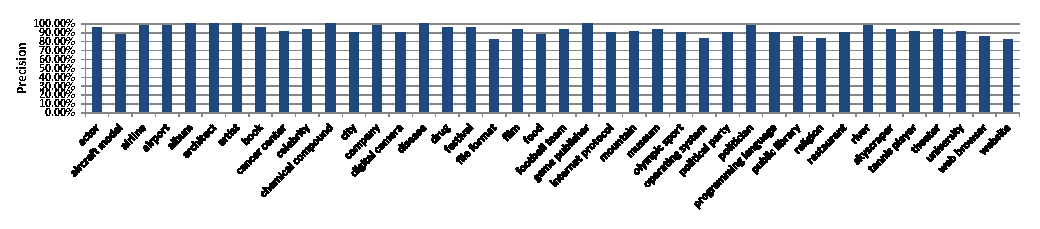
\includegraphics[width=\textwidth]{PrecNew-random50.eps}
\caption{Precision of randomly picked 50 instances over the benchmark concepts}
\label{fig:extract-precision-random}
\shrink
\end{figure*}

To estimate the correctness of the extracted \emph{isA} pairs,
we used the same benchmark as that in~\cite{WuLWZ12:Probase} with 40 concepts covering various domains (see Table~\ref{tab:stats:benchmark}). For each concept, to estimate its precision, we followed the same approach as in~\cite{WuLWZ12:Probase} by \emph{randomly} picking 50 instances and manually evaluating their correctness. The average precision of the \emph{isA} pairs over the benchmark concepts is 92.9\%, which is very close to that reported in~\cite{WuLWZ12:Probase}.
Figure~\ref{fig:extract-precision-random} further presents the precision of each individual concept.

\begin{table*}%[!ht]
\centering
\begin{tabular}{|l|l|}
\hline
{\bf Concept (\# of Instances)} & {\bf Representative Instances} \\
\hline \hline
actor (20226)& Tom Hanks, Marlon Brando, George Clooney\\
\hline
aircraft model	(160) & Airbus A320-200, Piper PA-32, Beech-18\\
\hline
airline (3929) & British Airways, Deltae\\
\hline
airport (3299) & Heathrow, Gatwick, Stansted\\
\hline
album (8377) & Thriller, Big Calm, Dirty Mind \\
\hline
architect (2825) & Frank Gehry, Le Corbusier, Zaha Hadid\\
\hline
artist (179724)	& Picasso, Bob Dylan, Madonna\\
\hline
book (63868) &	Bible,	Harry Potter, Treasure Island\\
\hline
cancer center (110) & Fox Chase, Care Alliance, Dana-Farber\\
\hline
celebrity	(32220) & Madonna, Paris Hilton, Angelina Jolie\\
\hline
chemical compound (339) & carbon dioxide, phenanthrene, carbon monoxide\\
\hline
city (48357) & New York,	Chicago,	Los Angeles\\
\hline
company (356136) &	IBM,	Microsoft,	Google\\
\hline
digital camera (802) &	Canon,	Nikon,	Olympus\\
\hline
disease (58017) & AIDS,	Alzheimer,	chlamydia\\
\hline
drug (32557) & tobacco,	heroin,	alcohol\\
\hline
festival (13252)	& Sundance,	Christmas,	Diwali\\
\hline
file format (3547) & PDF,	JPEG,	TIFF\\
\hline
film (73897) &	Blade Runner,	Star Wars,	Clueless\\
\hline
food (69836) & beef,	dairy,	French fries\\
\hline
football team (442)	& Real Madrid,	AC Milan,	Manchester United\\
\hline
game publisher	(337) & Electronic Arts,	Ubisoft,	Eidos\\
\hline
internet protocol (479) & HTTP,	FTP,	SMTP\\
\hline
mountain (1977) &	Everest,	the Alps,	the Himalayas\\
\hline
museum  (7314) & the Louvre, Smithsonian, the Guggenheim\\
\hline
olympic sport (331) & gymnastics,	athletics,	cycling\\
\hline
operating system (6164) & Linux, Solaris,	Microsoft Windows\\
\hline
political party (2012)	& NLD, ANC,	Awami League\\
\hline
politician (6065) &	Barack Obama,	Bush,	Tony Blair\\
\hline
programming language (2472)	& Java,	Perl,	PHP\\
\hline
public library (153) & Haringey, Calcutta,	Norwich\\
\hline
religion (3830) & Christianity,	Islam,	Buddhism\\
\hline
restaurant (28651) & Burger King,	Red Lobster,	McDonalds\\
\hline
river (6379)	& Mississippi,the Nile,	Ganges \\
\hline
skyscraper	(132) &	the Empire State Building,	the Sears Tower,	Burj Dubai\\
\hline
tennis player (281) & Maria Sharapova,	Andre Agassi, Roger Federer\\
\hline
theater (4174) & Metro,	Pacific Place,	Criterion\\
\hline
university (9954) &	Harvard,	Stanford,	Yale\\
\hline
web browser (1182)	& Internet Explorer,	Firefox,	Safari\\
\hline
website (34539) & YouTube,	Facebook,	MySpace\\
\hline
\end{tabular}
\caption{Benchmark concepts}
\label{tab:stats:benchmark}
\vskip -5ex
\end{table*}

In Table~\ref{tab:iterPrec}, we further examined the precision of the pairs extracted in round $i$ ($P_i$) and the overall precision of the pairs extracted from round $1$ to round $i$ ($Q_i$). Here $P_i$ and $Q_i$ are evaluated based on the duplicated pairs (i.e., $\Delta_i$). We notice that the overall precision when the iteration ends (i.e., $Q_{11}=93.95\%$) is higher than the 92.9\% precision reported above, because the 92.9\% precision was based on unique pairs. (Due to the high precision, double-counting the duplicates can increase the overall precision.)

Notice that we again have some trade-off between precision and recall here. As suggested by Table~\ref{tab:iterPrec}, $P_i$ drops as the iteration proceeds while we indeed extract more valid pairs. Again, the trade-off depends on how the information is utilized by the users. If precision is more important, we can stop the iteration earlier, while we can iterate for more rounds if recall is crucial. Nonetheless, a nice property of our framework is that the overall precision $Q_i$ is guaranteed to be good by the time the algorithm converges.

\begin{table}[H]
\small
\centering
\begin{tabular}{|r|r|r|r|}
  \hline
Round $i$ & $|\Delta_i|$ & $P_i$ & $Q_i$ \\
 \hline\hline
1   & 26,492,477 & 0.9728 & 0.9728\\
2	& 244,880,870 & 0.9713 & 0.9714\\
3	& 48,582,780 & 0.8877 & 0.9587\\
4	& 16,214,502 & 0.7976 & 0.9509\\
5	& 7,069,892 & 0.6846 & 0.9454\\
6	& 2,204,261 & 0.5403 & 0.9429\\
7	& 1,619,613 & 0.4378 & 0.9405\\
8	& 523,076 & 0.5 & 0.9398\\
9	& 106,641 & 0.3983 & 0.9397\\
10	& 51,644 & 0.3576 & 0.9396\\
11	& 23,113 & 0.3049 & 0.9395\\
  \hline
\end{tabular}
\caption{Precision of the pairs extracted}
\label{tab:iterPrec}
\vskip -4ex
\end{table}

Finally, we find that the overall precision shown in Table~\ref{tab:iterPrec} matches our lower bound developed in Section~\ref{sec:analysis:precision} quite well. According to Theorem~\ref{theorem:prec}, the overall precision
$P\geq\frac{2}{2+\alpha}P_2$. According to Table~\ref{tab:iterPrec}, we have $\alpha=\frac{|\Delta_1|}{|\Delta_2|}\approx 0.1082$. Hence, the predicted $P\geq 0.9487 P_2\approx 0.9215$, which is very close to the actual overall precision observed (i.e., $Q_{11}=0.9395$).

\subsection{Recall}

Evaluation of recall is challenging. Specifically, the recall is defined as:
\begin{equation}\label{eq:recall}
recall=\frac{\textrm{\# of valid isA pairs extracted}}{\textrm{\# of valid isA pairs in the corpus}}.
\end{equation}
Although computing the numerator is straightforward given that we have already evaluated the precision, estimating the denominator is an extremely hard problem. 
If we just count the number of distinct valid pairs from some sample sentences and try to scale up the estimate based on that, we cannot make the estimate reasonably accurate unless the sample size is sufficiently large. In fact, this problem of estimating the number of distinct values in a population is well known as ``\emph{estimating the number of species}'' in statistical literature~\cite{distinctSurvey}, and it has been shown that the estimation error cannot be bounded unless the sample size is $O(n)$, where $n$ is the population size~\cite{sample00}. Since our corpus contains billions of sentences, it means that we need to manually identify valid pairs from billions of sample sentences, which is clearly prohibitive. Perhaps because of this difficulty, so far we are not aware of any previous work on open-domain information extraction that reported recall as defined by Equation~\ref{eq:recall}.

Nonetheless, we further conducted experiments to evaluate ``recall'' based on the idea of sampling random sentences from the corpus.
We randomly sampled 400 sentences from our corpus that the algorithm extracted at least one pair, and manually identified the correct super-concepts and sub-concepts. We then measured the precision and recall based on the extracted pairs and the ground truth.

\begin{figure}[th]
\centering
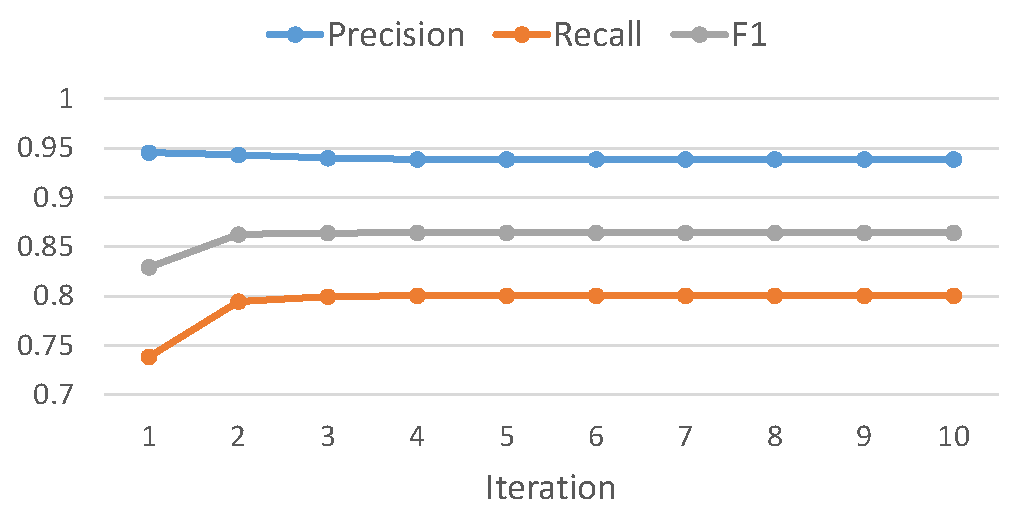
\includegraphics[width=\columnwidth]{random-sentence-eval.eps}
\caption{Precision, recall, and F1 score over 400 random sample sentences}
\label{fig:sentence:eval}
\shrink
\end{figure}

Figure~\ref{fig:sentence:eval} presents the results (as well as the F1 scores).
We observe that, while the algorithm can achieve high precision (close to 94\% when it terminates), the ``recall'' is relatively low (around 80\%, which gives an F1 score of 86\%). Note that, here the ``recall'' only means recall on this sample corpus, and we cannot make any inference on the recall over the whole corpus because of the aforementioned hardness result. 
However, in our experiments we do find that the algorithm does not perform well on rare sentences that contain many sub-concepts, usually because the algorithm cannot find enough evidence (i.e., sufficiently high frequency) for a boundary sub-concept that is close to the end of the sub-concept list.
In this sense, the current version of \emph{DetectSub} is a bit conservative.
We leave improving recall as one of the main directions for future work.


\section{Discussion and Critiques}

In this section, we would like to discuss and give some critiques to the applicability and extensibility of the analysis presented in this paper.

First, in our analysis, we have employed several assumptions, some of which may not always hold in practice.
The goal of the theoretical analysis in this paper is not to capture all real-world subtleties: such a model might be too complicated to be tractable for a formal analysis.
For example, when analyzing the efficiency of Algorithm~\ref{alg:HH2}, rather than assuming a uniform distribution (Assumption~\ref{assumption:uniform}), we could instead assume that the probability of a $y\in\Delta_i^x$ being the $y_k$ follows some distribution $\Pr(y)$.
But then we have to assume $\Pr(y)$ be certain known distribution (e.g., Gaussian) to make any further inference, which might still be unrealistic.
Hence, rather than developing sophisticated models which might provide better insights but also be difficult to understand, our intention in this paper is to provide a simple, basic model and show what we can infer by just using this model.
Our evaluation on a real data set shows that the results we derive from the model match the experimental observations, which substantiates the usefulness of the model.
Of course, it remains interesting to further explore possible extensions to the current model to make it more general.

Second, while the analysis in the paper is dedicated to the approach in~\cite{WuLWZ12:Probase}, it may also be applied to other cases.
Note that the approach in~\cite{WuLWZ12:Probase} can be used to extract other types of relations (e.g., ``part-of'' relations~\cite{PonzettoS07}), provided that there are patterns bearing the properties stated in Section~\ref{sec:extract:properties}.
Perhaps more importantly, similar analysis may be done for other bootstrapping procedures, which are popular in modern information extraction systems.
Indeed, this is an essential motivation of this paper, which, we hope, provides an example and makes a first step towards this direction.
However, Algorithm~\ref{alg:HH2} is not really a prototypical algorithm used in ``syntactic bootstrapping'' approaches. Typically, some candidate scoring functions are used to decide if an extraction is correct~\cite{BlohmCS07}.
The idea is to harvest more tuples with the current patterns, and expand the patterns by using the new tuples found.
This is essentially more complicated compared with semantic bootstrapping analyzed in this paper.
Because the set of patterns can change as syntactic bootstrapping proceeds, it is expected that there are more rounds of iterations.
Meanwhile, the overall precision does not only depend on the precision of the tuples in the bootstrapping phase: it also depends on the quality of the patterns extracted (and vice versa) in later rounds.
It is very interesting future work to see if the current framework we used for the analysis of semantic bootstrapping can be extended to analyze syntactic bootstrapping.

Third, one might also have the question regarding the implication and usefulness of such theoretical analysis. 
The meaning is that it will guide people on how to use semantic bootstrapping in practice. 
For example, our analysis suggests that we can trade off between precision and recall by using different iterations. 
As another example, as suggested by Theorem~\ref{theorem:prec}, the overall precision highly depends on the precision of the first two iterations.
Therefore, to improve the quality of the extracted pairs, one should focus on improving the quality of the pairs extracted in the first two iterations.
For instance, one may want to choose larger thresholds (used by \emph{DetectSuper} and \emph{DetectSub}) in the first two iterations and smaller thresholds in later iterations. As an alternative, one may also incorporate external, clean knowledge (e.g., \emph{isA} relations from \emph{WordNet}~\cite{wordnet} or \emph{Freebase}~\cite{freebase}) into the first two iterations to boost the precision.


\section{Related Work}\label{sec:relatedwork}

Automatically extracting relations from text corpus has been studied for decades. Early work focused on information extraction from a
\emph{closed} domain (e.g., news). These systems usually used supervised learning approaches such as Hidden Markov Models (e.g.,~\cite{FreitagM00-HMM}), 
rule learning (e.g.,~\cite{Soderland99-rule}), or Conditional Random Fields (e.g.~\cite{McCallum03-CRF}), which were elaborately tuned for that specific domain. As a result, while these approaches might be effective on  documents that are similar to those in the training corpus, it is difficult to apply them to \emph{open} domains like the whole Web, where the corpus and the target relations are much more diverse.

To the best of our knowledge, the first work towards \emph{open} domain information extraction was DIPRE~\cite{brin98},
which leveraged the basic idea of \emph{syntactic bootstrapping}. Similar ideas were adopted by several later work
(e.g.,~\cite{Agichtein-snowball00,PascaLBLJ06,RiloffJ99-multi-bootstrap}).
However, these systems usually require substantial human effort to provide manually tagged \emph{seed} instances for every target
relation. KnowItAll~\cite{EtzioniCDKPSSWY04} partially alleviated this practical challenge by specifying \emph{seed} patterns
(or rules) instead of seed instances. But this raised a new question about the availability of hand-crafted linguistic patterns.
TextRunner~\cite{BankoCSBE07} later addressed this issue by using a self-supervised learner to automatically identify extraction
patterns. Recent work~\cite{FaderSE11-reverb} further improved TextRunner by enforcing certain syntactic constraints to suppress
incoherent and uninformative extractions. Nonetheless, the precision and scale of the extracted relations remains an issue.
Another prominent recent work was the NELL project~\cite{NELL}, which viewed information extraction as a multi-task learning problem
and employed semi-supervised learning methods. However, NELL still uses syntactic bootstrapping and requires \emph{seed}
instances for the learners to bootstrap with. As a result, it suffers similar problems.

Unlike this line of work on syntactic bootstrapping, Probase~\cite{WuLWZ12:Probase} applied the idea of \emph{semantic bootstrapping} to \emph{isA} relation extraction and showed promising performance.
Nonetheless, it only gave empirical results with no performance guarantee.
This paper serves as a companion of~\cite{WuLWZ12:Probase}.
We have conducted a detailed theoretical analysis that further explains the working mechanism underlying semantic bootstrapping.
So far, we are not aware of similar study on any previous \emph{isA} relation extraction algorithm.
It is our hope that our work in this paper could inspire future research on formal analysis of information extraction systems.

On the other hand, semantic bootstrapping does not address the issue of how to obtain high-quality syntactic patterns.
There has also been a lot of work on how to obtain good syntactic patterns. For example, Riloff and Jones~\cite{RiloffJ99-multi-bootstrap} proposed a \emph{multi-level bootstrapping} architecture, by introducing a \emph{meta-bootstrapping} stage before the standard syntactic bootstrapping framework. Patwardhan and Riloff~\cite{PatwardhanR07-pattern-affinity} built a classifier that can evaluate the relevance of an extraction pattern to a piece of text in the corpus. Semantic bootstrapping is orthogonal to this line of work. It is interesting future work to combine both to develop a perhaps more powerful system that consists of two layers: the bottom layer is syntactic bootstrapping, whose output is a set of high-quality extraction patterns; the top layer is semantic bootstrapping, whose input is the output from syntactic bootstrapping, and whose output is the high-quality pairs extracted. This architecture is visualized in Figure~\ref{fig:two-layer}.

\begin{figure}[th]
\centering
\includegraphics[width=\columnwidth]{two-layer.eps}
\caption{Combine syntactic and semantic bootstrapping}
\label{fig:two-layer}
\shrink
\end{figure}

Finally, it is worth mentioning that semantics-based techniques have been studied for decades in natural language processing (NLP) research, as were detailed in the recent survey by Cambria and White~\cite{CambriaW14}.
Unlike pure syntax-based approaches which basically adopt a ``bag-of-words'' model, semantics-based approaches take a ``bag-of-concepts'' view that focuses on detecting the intrinsic meaning underlying the text.
Knowledge representation lies in the center of these semantics-based approaches, with the aim of building universal taxonomies or Web ontologies~\cite{CambriaW14}.
Except for the effort on automatically extracting worldly facts from large open-domain corpus that has been elaborated extensively throughout this paper, there are also many other popular Semantic Web projects (e.g., Annotea~\cite{KahanK01}, SIOC~\cite{BreslinHBD05}, and SKOS~\cite{BakerBIMSS13}).
Researchers have also been attempting semantics-based techniques that go beyond encoding subsumption knowledge in taxonomies and ontologies.
For example, there is a recent move towards \emph{sentic computing}~\cite{cambria2012sentic}, which presents an approach to concept-level sentiment analysis based on graph mining and dimensionality reduction techniques.
Incorporating richer knowledge and semantics into semantic bootstrapping will be a very interesting direction for future work.

\section{Conclusion}\label{sec:conclusion}

In this paper, we revisited a semantic bootstrapping framework for open-domain \emph{isA} relation extraction that differs from previous work based on syntactic bootstrapping. Rather than seeking more and more syntactic patterns as the iteration proceeds, semantic bootstrapping uses a fixed set of patterns and leverages the knowledge identified in previous rounds to help extract more knowledge. We gave both theoretical and empirical study of its performance. We demonstrate that semantic bootstrapping can indeed achieve very high precision while retaining good recall on large-scale corpus.


{
\renewcommand{\baselinestretch}{1.1}
\small

\bibliographystyle{abbrv}
\bibliography{semanticIE}
}

\begin{minipage}{3.5in}
\vspace*{-5mm}
\begin{IEEEbiography}
[{\includegraphics[width=1in,height=1.25in,clip,keepaspectratio]{wu.jpg}}]
  {Wentao Wu} received the B.S. and M.S. degrees in computer science from Fudan
  University in 2007 and 2010, respectively, and the Ph.D. degree from the University
  of Wisconsin-Madison in 2015. He is currently a researcher at the Data Management, Exploration and Mining (DMX) group, Microsoft Research, Redmond.
  His research interest includes database management systems, distributed systems, big data analytics, data mining, and etc.

\end{IEEEbiography}\vspace{-10mm}
\begin{IEEEbiography}
[{\includegraphics[width=1in,height=1.25in,clip,keepaspectratio]{li.jpg}}]
  {Hongsong Li} received the Ph.D. degree from Beijing Jiaotong University, majored in computer science.
  He joined Microsoft Research Asia as an associate researcher in 2006.
  He has been with the Data intelligence and Tool Group, the Web Search and Mining Group, and the Data Management, Analytics and Services Group (DMAS).
  His research interests include knowledge base, web data mining, machine learning, and natural language processing.
\end{IEEEbiography}\vspace{-10mm}
\begin{IEEEbiography}
[{\includegraphics[width=1in,height=1.25in,clip,keepaspectratio]{wang.jpg}}]
  {Haixun Wang} received the BS and MS degrees
in computer science from Shanghai Jiao Tong
University in 1994 and 1996, respectively, and
the PhD degree in computer science from the
University of California in 2000. He joined Google
Research, Mountain View, in 2013. From 2009 to
2013, he was with Microsoft Research, Asia,
where he led the database team. From 2000 to
2009, he was with IBM Research, Watson. His
research interests are in text analytics, semantic
network and knowledge base, etc.
\end{IEEEbiography}\vspace{-10mm}
\begin{IEEEbiography}
[{\includegraphics[width=1in,height=1.25in,clip,keepaspectratio]{zhu.jpg}}]
  {Kenny Q. Zhu} graduated with the BEng degree
in electrical engineering in 1999 and the PhD
degree in computer science in 2005 from
National University of Singapore. He is a
professor of Computer Science at 
Shanghai Jiao Tong University.
From 2007 to 2009, he was a postdoctoral
researcher at Princeton University. His research
interests are text mining, natural language understanding 
and knowledge discovery, and are partially supported by
NSFC and Google Faculty Award.
\end{IEEEbiography}
\end{minipage}

\end{document}

